%%%% methodologie_donnees.tex
%%%% Data Challenge Burkina 2026, édition Éducation, défi 1 : méthodologie de collecte et de nettoyage
%%%% Mise en page reprise du gabarit de la note d'intention.
%%%% Évaluation anonyme : ne mettre aucun nom, aucune affiliation, aucun lien personnel.

\documentclass{article}
\pdfpagewidth=8.5in
\pdfpageheight=11in

\usepackage{ijcai26}

\usepackage{times}
\usepackage{url}
\usepackage[utf8]{inputenc}
\usepackage[T1]{fontenc}
\usepackage[english,french]{babel}
\usepackage{xcolor}
\usepackage{xurl}
\usepackage[colorlinks=true,
            citecolor=blue!70!black,
            linkcolor=red!60!black,
            urlcolor=blue!70!black,
            pdfauthor={},
            pdftitle={Sentinelle Scolaire : méthodologie de collecte et de nettoyage des données},
            pdfcreator={},
            pdfproducer={}]{hyperref}
\usepackage[small]{caption}
\usepackage{graphicx}
\usepackage{amsmath}
\usepackage{booktabs}
\usepackage{tabularx}
\usepackage{array}
\usepackage{float}
\usepackage{placeins}

\urlstyle{same}
\emergencystretch=1.5em
\graphicspath{{figures/}}

\addto\captionsfrench{%
  \renewcommand{\tablename}{Tableau}%
  \renewcommand{\figurename}{Figure}%
  \renewcommand{\refname}{Références}%
}

\newcommand{\sol}{Sentinelle Scolaire}
\newcolumntype{L}[1]{>{\raggedright\arraybackslash}p{#1}}
\newcolumntype{Y}{>{\raggedright\arraybackslash}X}

\pdfinfo{
/TemplateVersion (IJCAI.2026.0)
}

\title{\sol{}\\[3pt]
{\large\mdseries Méthodologie de collecte et de nettoyage des données}}
\author{
Data Challenge Burkina 2026, édition Éducation, défi 1\\
\affiliations
Documentation technique, étapes 01 (collecte) et 02 (nettoyage)
}

\begin{document}
\renewcommand{\tablename}{Tableau}\renewcommand{\figurename}{Figure}\renewcommand{\refname}{Références}
\raggedbottom

\maketitle
\thispagestyle{plain}
\pagestyle{plain}

%======================================================================
\section{Objet et principes}
%======================================================================

Ce document décrit comment les données de \sol{} ont été rassemblées puis nettoyées, avant toute modélisation. Il couvre les deux premières étapes du parcours des données fixé par le challenge~\cite{dcb_document} : la collecte (dépôt 01) et le nettoyage (dépôt 02). Il dit quels fichiers ont été exploités, lesquels ont été écartés et pourquoi, quelles corrections ont été apportées et comment chacune peut être vérifiée.

Quatre principes guident ces deux étapes.

\textbf{Des données officielles uniquement.} Toutes les données proviennent des fichiers remis par les organisateurs : la base principale de la DGESS~\cite{dgess_base} et le Data Pack~\cite{dcb_guide}. Aucune donnée n'a été inventée, et aucune valeur manquante n'a été remplacée par une valeur plausible sans le dire. Les données simulées qui illustraient le prototype de la note d'intention ne sont jamais utilisées.

\textbf{Des originaux intacts.} Les fichiers des organisateurs sont en lecture seule : le code refuse d'écrire dans leur dossier. Une copie d'archive a été faite avant tout traitement, et la taille de chacun des 167 fichiers du Data Pack a été comparée au manifeste de téléchargement : tous sont conformes.

\textbf{Une traçabilité jusqu'à la page.} Chaque valeur de la base garde son fichier d'origine, sa page et, pour les tableaux extraits de PDF, sa ligne. Chaque fichier source est identifié par son empreinte SHA-256 et son adresse de téléchargement d'origine. Toute correction est consignée dans un journal.

\textbf{Une chaîne reproductible.} Chaque étape est un module Python (\texttt{sentinelle.collecte}, \texttt{sentinelle.nettoyage}) présenté par un notebook exécuté. Une seule commande relance chaque étape et régénère ses dépôts, sans aucune intervention manuelle.

%======================================================================
\section{Les sources exploitées}
%======================================================================

\subsection{Ce que les organisateurs ont remis}

Le dossier remis contient 347 fichiers : 173 fichiers sources (138 PDF, 23 classeurs Excel, des archives cartographiques et quelques fichiers de documentation) et 174 extractions au format CSV préparées par les organisateurs. La base principale de la DGESS couvre les 13 anciennes régions de 2015-2016 à 2024-2025 : effectifs, nouveaux inscrits, taux d'admission, de scolarisation et d'achèvement, réussite au CEP, indices de parité et nombre d'écoles. Elle ne contient ni taux d'abandon, ni redoublement, ni données provinciales. Ces informations, indispensables au défi, se trouvent dans les annuaires du Data Pack.

\subsection{Les sources retenues}

Chaque fichier source a été examiné. 146 sont retenus et répartis en 36 jeux de données selon leur rôle dans le défi (tableau~\ref{tab:sources}). Les annuaires de la DGESS fournissent la variable cible : les taux de promotion, de redoublement et d'abandon par province, classe et sexe, pour huit éditions, et l'historique des effectifs et des redoublants qui permet de recalculer ces taux~\cite{dgess_annuaires}. Les annuaires de l'éducation non formelle décrivent l'autre versant du décrochage : les centres qui accueillent les adolescents non scolarisés ou déscolarisés ; ceux du préscolaire mesurent la préparation à l'entrée au CP1. Les rapports du ST-ESU et les situations de déplacés internes du CONASUR mesurent l'exposition à la crise sécuritaire~\cite{stesu,conasur}. Les publications de l'INSD décrivent le contexte démographique et social~\cite{insd_rgph,insd_annuaires,insd_pauvrete,ehcvm2021,eds2021}. Les limites administratives COD-AB servent de référentiel géographique et de fond de carte~\cite{codab}.

\begin{table*}[!t]
\centering
\small
\begin{tabularx}{\textwidth}{@{}L{3.3cm} Y L{2.6cm} L{2.4cm} L{3.4cm}@{}}
\toprule
Source & Contenu retenu & Période & Niveau & Usage dans \sol{} \\
\midrule
Base principale DGESS~\cite{dgess_base} & Préscolaire et primaire : effectifs, admission, scolarisation, achèvement, CEP, parité, écoles, structures et salles (14 feuilles, 21 tableaux) & 2015-2016 à 2024-2025 & 13 régions & Lue en entier ; contexte régional du modèle, contrôle des totaux \\
Annuaires du primaire DGESS (8)~\cite{dgess_annuaires} & Taux de promotion, redoublement, abandon ; effectifs et redoublants ; écoles, salles, maîtres ; distance ; CEP ; 43 communes prioritaires & Éditions 2017-2018 à 2024-2025 & 45 provinces, communes & Variable cible, offre scolaire \\
Annuaires de l'éducation non formelle DGESS (5, dont un doublon)~\cite{dgess_annuaires} & Centres et apprenants, adultes et adolescents, par milieu & Campagnes 2018, 2019, 2020, 2024 & 45 provinces & Seconde chance des déscolarisés \\
Annuaires du préscolaire DGESS (2)~\cite{dgess_annuaires} & Taux de préscolarisation, enfants par section & 2023-2024, 2024-2025 & 45 provinces & Préparation à l'école \\
Tableaux de bord, synthèses, dépliants DGESS (42)~\cite{dgess_tdb} & Séries régionales d'indicateurs, chiffres clés nationaux & 2015-2016 à 2023-2024 & Région, pays & Recoupement, contrôle des totaux \\
Rapports mensuels ST-ESU (24)~\cite{stesu} & Écoles fermées et rouvertes, élèves et enseignants concernés & Nov. 2021 à fév. 2026 & Région, province & Exposition sécuritaire \\
Déplacés internes CONASUR (20 classeurs)~\cite{conasur} & Déplacés et enfants déplacés accueillis & Janv. 2019 à mai 2025 & Commune & Pression d'accueil, départs \\
Annuaires régionaux INSD 2024 (10)~\cite{insd_annuaires} & Écoles, salles, salles sous paillote, élèves, enseignants & Environ 2014 à 2024 & Commune & Variables communales \\
Annuaires nationaux INSD (10)~\cite{insd_annuaires} & Pages sur l'enseignement primaire ; édition 2024 en 17 régions & 2015 à 2024 & Région & Recoupement \\
RGPH 2019 (5 publications)~\cite{insd_rgph} & Pauvreté et disparités par commune, scolarisation, population par localité, projections & 2019 à 2035 & Commune, localité & Contexte, dénominateurs \\
Pauvreté et conditions de vie~\cite{insd_pauvrete,ehcvm2021,eds2021} & Profils régionaux de pauvreté, tableau de bord social, EHCVM 2021, EDS 2021 (mariage précoce) & 2020 à 2024 & Région, province & Contexte \\
Limites COD-AB~\cite{codab} & 351 communes avec ancien et nouveau P-code, provinces, régions & Août 2025 & Commune & Référentiel, cartes \\
Écoles OpenStreetMap~\cite{hotosm} & 11\,974 structures éducatives géolocalisées & Nov. 2026 & Point & Localisation, noms anciens \\
Séries Banque mondiale~\cite{bm_unesco} & Indicateurs nationaux d'éducation & 1970 à 2025 & Pays & Cohérence des agrégats \\
\bottomrule
\end{tabularx}
\caption{Sources exploitées, regroupées par producteur. Entre parenthèses : nombre de fichiers. Source : fichiers remis par les organisateurs ; classement des auteurs.}
\label{tab:sources}
\end{table*}

\subsection{Les sources écartées}

Les 27 fichiers non retenus le sont pour une raison écrite dans le bilan des sources déposé avec la collecte (tableau~\ref{tab:ecartees}). Aucun fichier n'est resté sans décision. L'éducation non formelle et le préscolaire, d'abord jugés hors du champ du primaire, ont été réintégrés : l'une accueille les enfants sortis de l'école, l'autre prépare leur entrée. Les géométries sont réservées à l'étape cartographique, et les documents méthodologiques sont cités mais ne contiennent pas de tableau à extraire.

\begin{table}[!t]
\centering
\small
\begin{tabularx}{\columnwidth}{@{}Y r@{}}
\toprule
Motif d'exclusion & Fichiers \\
\midrule
Géométries et métadonnées cartographiques, réservées aux cartes & 9 \\
Documentation du challenge et du Data Pack & 5 \\
Résultats généraux du RGPH, repris plus finement ailleurs & 4 \\
ONG, supérieur, emploi, doublons, documents de méthode & 9 \\
\midrule
Total & 27 \\
\bottomrule
\end{tabularx}
\caption{Fichiers sources écartés et motifs. Source : bilan des sources, calculs des auteurs.}
\label{tab:ecartees}
\end{table}

%======================================================================
\section{Méthode de collecte}
%======================================================================

\subsection{Un catalogue déclaratif}

La collecte part d'un catalogue qui déclare, pour chaque jeu de données, les fichiers concernés et une règle de sélection des pages. Les lignes retenues sont copiées sans aucune modification : la remise en forme relève du nettoyage. Trois règles suffisent :
\begin{itemize}
\item \emph{fichier entier}, pour les classeurs Excel et les documents courts ;
\item \emph{en-tête de page}, pour les annuaires de la DGESS : une page est retenue si ses quatre premières lignes portent l'intitulé de la section (par exemple « TAUX DE PROMOTION, REDOUBLEMENT »). Les numéros de page changent d'une édition à l'autre, mais l'intitulé reste stable ;
\item \emph{texte de la page}, pour les annuaires régionaux de l'INSD, dont la numérotation des tableaux diffère d'une région à l'autre : une page est retenue si l'une de ses lignes associe le primaire et la commune, hors table des matières. Les pages de suite sans titre sont rattachées au tableau qui précède.
\end{itemize}

\subsection{Traçabilité et contrôle de couverture}

Chaque ligne extraite porte son fichier d'origine, son CSV du Data Pack et sa période. La période est lue dans le nom du fichier ; quand ce nom ne la donne pas, elle est relevée dans le document lui-même et documentée dans le code. Un registre des sources décrit chaque fichier utilisé : pages retenues, nombre de lignes, empreinte SHA-256 du fichier d'origine et de son extraction, producteur, adresse de téléchargement et date de collecte.

Un contrôle de couverture vérifie que chaque fichier d'un jeu sélectif fournit des pages, et que le volume extrait reste comparable d'une année à l'autre. Il a permis de repérer qu'une section n'existait que dans certaines éditions (les 43 communes prioritaires, de 2017-2018 à 2020-2021) et d'expliquer un volume plus faible en 2017-2018 : cette édition ne publie pas de totaux régionaux pour les taux de flux, sans qu'aucune donnée provinciale ne manque.

\subsection{Résultat}

La collecte produit 36 jeux de données issus de 146 fichiers sources, soit 455\,372 lignes extraites, ainsi qu'un inventaire des 347 fichiers remis, le bilan des sources retenues et écartées, le registre et le contrôle de couverture. Les 40 fichiers du dépôt 01 suivent la convention de nommage du challenge, avec un LISEZ-MOI.

%======================================================================
\section{Méthode de nettoyage}
%======================================================================

Le nettoyage transforme les extractions, encore au format des PDF (en-têtes sur plusieurs lignes, noms de région en titre de bloc, lignes de total, virgule décimale), en tables longues : une valeur par ligne, avec son entité, sa période, sa classe, son sexe et son origine.

\subsection{Un référentiel géographique à deux découpages}

En juillet 2025, le pays est passé de 13 à 17 régions et de 45 à 47 provinces. Toutes les données de la DGESS suivent l'ancien découpage, alors que les décideurs raisonnent désormais dans le nouveau. La commune sert de pivot : chacune des 351 communes COD-AB porte son P-code actuel et son ancien P-code, dont les quatre et six premiers caractères désignent l'ancienne région et l'ancienne province~\cite{codab}. Les noms des anciennes entités, absents de COD-AB, sont repris du fichier OpenStreetMap, qui suit l'ancien découpage avec ses P-codes~\cite{hotosm}.

Les couches des cinq niveaux sont obtenues en regroupant les contours des communes, ce qui garantit des limites identiques d'un niveau à l'autre (figure~\ref{fig:decoupages}). Le passage d'un découpage à l'autre est simple : 43 anciennes provinces correspondent chacune à une seule province de 2025, seules deux ont été scindées (le Soum, entre Djelgodji et Karo-Peli ; la Tapoa, entre Dyamongou et Gobnangou), et aucune province de 2025 ne regroupe plusieurs anciennes. Trois provinces ont seulement changé de nom (Sanmatenga, Oubritenga, Kossi). Pour le prototype web, les contours sont simplifiés par une méthode qui préserve la mosaïque, sans trou ni chevauchement entre entités : la couche des provinces passe de 17\,Mo à 133\,Ko.

\begin{figure*}[t]
\centering
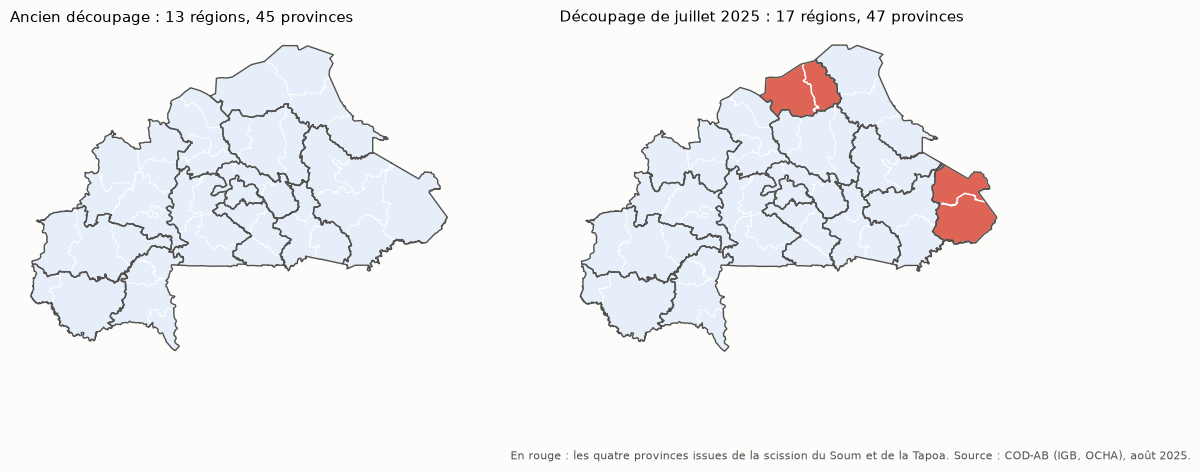
\includegraphics[width=0.92\textwidth]{fig_decoupages.png}
\caption{Les deux découpages administratifs, reconstruits à partir des communes. En rouge : les quatre provinces issues de la scission du Soum et de la Tapoa. Source : COD-AB (IGB, OCHA), août 2025 ; mise en forme des auteurs.}
\label{fig:decoupages}
\end{figure*}

Une table d'alias relie chaque orthographe rencontrée au bon code (« Komondjari », « Komandjari », « LES BALE », « CASCADE », « PLATEAU CENTRAL »…). Les publications de la DGESS ne sont rapprochées que des noms de l'ancien découpage, pour éviter toute confusion avec le nouveau, où le Soum, par exemple, est devenu une région.

\subsection{Les tableaux des annuaires de la DGESS}

\textbf{Taux de flux.} Chaque province occupe trois lignes (promotion, redoublement, abandon), son nom figurant sur l'une d'elles, parfois coupé sur deux lignes ou collé au libellé dans la même cellule. Le lecteur regroupe ces trois lignes, reconstitue le nom et le rapproche de la table d'alias. La promotion et l'abandon couvrent le CP1 au CM1, le redoublement le CP1 au CM2.

\textbf{Effectifs et redoublants.} Chaque édition donne, pour chaque province, les dix dernières années, trois lignes par année (garçons, filles, total). L'extraction a parfois perdu, déformé ou dupliqué l'étiquette de l'année. Un bloc est donc lu en entier avant d'être daté : l'étiquette du PDF fait foi quand elle est valide et non répétée ; sinon l'année se déduit de l'étiquette voisine. Le journal consigne 13 années déduites, un groupe imprimé deux fois dans le PDF et retiré, et trois lignes intitulées « Somme de » dont le sexe est déduit de la position. Pour chaque année, la valeur retenue est celle de l'édition la plus récente, les éditions successives révisant parfois l'année en cours.

\textbf{Validation.} Les taux de promotion, de redoublement et d'abandon ont été recalculés à partir des effectifs et des redoublants (méthode de la cohorte reconstituée), en conservant les valeurs négatives que les annuaires ramènent à zéro. Comparés aux taux publiés, ils s'en écartent de 0,03 point en médiane, à condition de rattacher les taux d'une édition au passage de l'année précédente à celle de l'édition. Ce résultat valide à la fois la lecture des tableaux et la convention de calcul de la DGESS.

\subsection{La base principale de la DGESS}

Le classeur remis par les organisateurs est lu en entier : ses 14 feuilles empilent 21 tableaux selon trois mises en page (une colonne par année et le sexe en ligne ; trois colonnes garçons, filles, total sous chaque année ; une seule valeur par année pour les indices de parité, les structures et les salles). Chaque feuille est parcourue ligne par ligne : une ligne « Tableau » ouvre un tableau, l'en-tête donne les colonnes de libellés et les années, écrites de cinq façons (« 2015-2016 », « 2015/16 », « 2024/25 », ou l'année de fin seule, « 2016 », pour le préscolaire et le CEP). Les libellés sont reportés vers le bas (une région vaut pour les lignes de statut qui la suivent) et reconnus par vocabulaire : région, statut, milieu, classe, sexe, total. Une cellule d'en-tête qui porte un texte parasite après un saut de ligne n'est lue que sur sa première ligne ; les cellules isolées en bas de feuille, sans libellé, sont écartées. Le résultat, \texttt{fait\_base\_principale}, compte 6\,621 valeurs.

Pour chaque comptage, la somme des parties retrouve le total publié dans les 1\,691 cas vérifiés (régions et pays, garçons et filles, statuts, milieux, classes), et le taux d'achèvement national de 2024-2025 retrouve les 51,6\,\% cités dans la note d'intention. Les variations d'un facteur supérieur à 2,5 d'une année à l'autre (73 valeurs, presque toutes au préscolaire) sont consignées sans correction : en 2019-2020, plusieurs régions semblent avoir leurs structures privées et communautaires interverties, le total restant juste.

\subsection{L'éducation non formelle et le préscolaire}

Les annuaires de l'éducation non formelle donnent, par province et milieu, les centres des adultes et des adolescents et leurs apprenants (tableaux 1.1 et 1.3). La campagne est lue dans l'en-tête des pages, jamais dans le nom du fichier : deux fichiers du Data Pack, intitulés 2019 et 2021, sont identiques (même empreinte) et portent la campagne 2020, et celui intitulé 2020 porte la campagne 2019. Le doublon est écarté ; restent les campagnes 2018, 2019, 2020 et 2024, chacune pour les 45 provinces. Les deux tableaux se recoupent (adultes et adolescents retrouvent le total dans tous les cas), et la somme des provinces retrouve le total régional publié pour les 52 régions et campagnes.

Les annuaires du préscolaire 2023-2024 et 2024-2025 donnent, par province et sexe, la population préscolarisable, les enfants préscolarisés, le taux de préscolarisation et les enfants par section. Chaque entité occupe trois lignes ; le nom de la région, centré dans le PDF, tombe dans le bloc d'une province (« BOUCLE DU » puis « MOUHOUN » dans le bloc du Mouhoun), et le total régional n'est pas toujours intitulé. Chaque bloc est donc lu en entier : les noms de région en sont retirés, puis le reste est reconnu comme province ; un bloc sans province est le total de la région. Le tableau par section change de numéro d'une édition à l'autre et se reconnaît à son intitulé. Les sections retrouvent le total dans les 354 cas, et 24 totaux régionaux sur 26 sont identiques à ceux de la base principale.

\subsection{Les rapports du ST-ESU}

Les rapports mensuels donnent les écoles fermées et rouvertes par ordre d'enseignement, région et province. Seul le primaire est retenu. Deux niveaux de lecture coexistent. Au niveau provincial, chaque ligne est contrôlée (filles + garçons = total), et un rapport n'est jugé fiable que si la somme des provinces retrouve le total primaire publié à 5\,\% près : c'est le cas de 12 tableaux sur 30, issus des rapports en texte natif de novembre 2021 à mai 2022 et d'octobre 2023. Les rapports lus par reconnaissance de caractères sont conservés mais marqués non fiables. Au niveau régional, la phrase de synthèse de chaque région (« Est : 1\,090 établissements scolaires fermés, affectant 189\,095 élèves… ») résiste mieux à cette lecture et donne une série mensuelle des fermetures de novembre 2021 à mai 2023. À partir d'octobre 2023, les rapports ne recensent plus les fermetures, seulement les réouvertures.

\subsection{Les déplacés internes}

Deux formats coexistent : des fichiers détaillés par site d'accueil, avec P-codes, et des synthèses par commune, sans code. Le P-code est utilisé quand il existe ; sinon la commune est rapprochée par son nom, avec la province pour lever les homonymies, puis par l'orthographe la plus proche dans la même province (367 rapprochements), enfin par une courte table de correspondance documentée ; les arrondissements de Ouagadougou sont rattachés à la commune. Seules restent non rapprochées des lignes de total. Quand deux fichiers décrivent la même date, la version « après nettoyage » du CONASUR est préférée. Les enfants déplacés, non recensés séparément avant septembre 2021, sont laissés vides plutôt que mis à zéro. La série obtenue couvre 328 communes et 46 dates, de janvier 2019 à mars 2023 ; son dernier total, 2\,062\,534 personnes, correspond au chiffre publié pour cette date (figure~\ref{fig:pdi}).

\begin{figure}[!t]
\centering
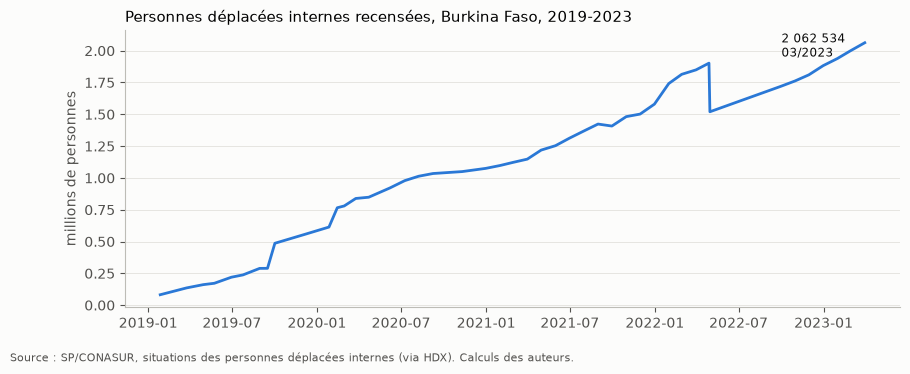
\includegraphics[width=\columnwidth]{fig_pdi.png}
\caption{Personnes déplacées internes recensées, 2019-2023. La chute d'avril 2022 vient d'un fichier incomplet, traité à l'étape suivante. Source : SP/CONASUR via HDX ; calculs des auteurs.}
\label{fig:pdi}
\end{figure}

%======================================================================
\section{La base Sentinelle Scolaire}
%======================================================================

Le nettoyage produit une base unique au format GeoPackage, qui s'ouvre dans un logiciel de cartographie comme QGIS, et dont chaque table est aussi exportée en CSV (tableau~\ref{tab:base}). Elle suit un schéma en étoile : des couches et tables de référence, des tables de faits reliées par les P-codes et la période, et des tables de traçabilité. Deux tables de métadonnées la documentent : \texttt{meta\_tables} décrit chaque table (contenu, grain, clé, sources, période, nombre de lignes), et \texttt{meta\_variables} est le dictionnaire des 210 variables (type, unité, description). Un contrôle vérifie qu'aucune table ni variable ne reste sans description.

\begin{table*}[!t]
\centering
\small
\begin{tabularx}{\textwidth}{@{}L{4.1cm} Y L{3.6cm} r@{}}
\toprule
Table & Contenu & Grain & Lignes \\
\midrule
\multicolumn{4}{@{}l}{\emph{Couches cartographiques et référentiel}} \\
commune & Contours, P-codes et rattachements dans les deux découpages & commune & 351 \\
province, region & Découpage de juillet 2025 ; indication des provinces scindées & province, région & 47 ; 17 \\
province\_ancienne, region\_ancienne & Ancien découpage, utilisé par les données DGESS & province, région & 45 ; 13 \\
ref\_alias\_nom & Orthographes rencontrées et codes correspondants & nom & 72 \\
\multicolumn{4}{@{}l}{\emph{Tables de faits}} \\
fait\_flux\_publie & Taux de promotion, redoublement et abandon publiés & édition, entité, classe, sexe & 22\,032 \\
fait\_effectifs\_editions & Effectifs et redoublants tels que publiés dans chaque édition & édition, année, entité, classe, sexe & 101\,199 \\
fait\_effectifs\_retenus & Une valeur par année (édition la plus récente), fiabilité de la répartition par sexe & année, entité, classe, sexe & 20\,720 \\
fait\_offre\_province & Écoles, salles, maîtres, élèves et ratios d'encadrement & année, entité, statut & 1\,389 \\
fait\_enf\_province & Éducation non formelle : centres et apprenants & campagne, entité, milieu & 708 \\
fait\_prescolaire\_province & Préscolaire : taux, enfants par section & année, entité, sexe & 354 \\
fait\_base\_principale & Les 21 tableaux de la base principale (préscolaire et primaire) & tableau, entité, statut, milieu, classe, sexe, année & 6\,621 \\
fait\_esu\_province & Écoles primaires fermées et rouvertes, fiabilité du rapport & rapport, type, province & 389 \\
fait\_esu\_region & Établissements fermés, élèves et enseignants affectés & rapport, région & 77 \\
fait\_pdi\_commune & Déplacés internes et enfants déplacés & date, commune & 9\,989 \\
\multicolumn{4}{@{}l}{\emph{Métadonnées et traçabilité}} \\
meta\_tables, meta\_variables & Description des tables, dictionnaire des variables & table ; variable & 21 ; 210 \\
meta\_source & Registre des sources de la collecte & fichier, jeu & 191 \\
meta\_journal\_nettoyage & Corrections, déductions, rapprochements, lignes écartées & opération & 1\,179 \\
meta\_controles & Résultat des contrôles automatiques & contrôle & 23 \\
\bottomrule
\end{tabularx}
\caption{Tables de la base \sol{}. Source : calculs des auteurs à partir des fichiers remis par les organisateurs.}
\label{tab:base}
\end{table*}

%======================================================================
\section{Contrôles et résultats}
%======================================================================

Les contrôles sont automatiques et rejoués à chaque exécution (tableau~\ref{tab:controles}). Ils répondent aux règles du challenge : vérifier les totaux contre les publications d'origine et se méfier des découpages et des noms~\cite{dcb_document}. La première carte de l'abandon observé, établie dès que la jointure entre données et contours a fonctionné, en montre l'usage (figure~\ref{fig:abandon}).

\begin{table*}[!t]
\centering
\small
\begin{tabularx}{\textwidth}{@{}L{5.2cm} Y L{1.6cm}@{}}
\toprule
Contrôle & Résultat & Statut \\
\midrule
Complétude des taux de flux et des effectifs & 45 provinces sur 45 pour chacune des 8 éditions & Conforme \\
Jointure avec les contours & 45 provinces sur 45 trouvent leur contour, pour chaque année & Conforme \\
Garçons + filles = total & Aucun écart & Conforme \\
Somme des provinces = total national publié & Exacte pour 7 années sur 10 ; écart inférieur à 1\,\% en 2018-2019 et 2022-2023, dû aux révisions entre éditions & À noter \\
Somme des provinces = totaux régionaux publiés & 39 écarts supérieurs à 0,5\,\% sur 3\,236 comparaisons, expliqués par les révisions et l'anomalie de 2024-2025 & À noter \\
Répartition filles / garçons plausible & 31 provinces sur 45 hors de l'intervalle [0,8 ; 1,25] dans l'annuaire 2024-2025 ; seul le total est alors utilisable & Anomalie de la source \\
Taux recalculés et taux publiés & Écart médian de 0,03 point & Conforme \\
Rapports ESU : somme des provinces = total publié & 12 tableaux sur 30 à 5\,\% près ; les autres sont marqués non fiables & À noter \\
Déplacés internes rattachés à une commune & 328 communes, 46 dates ; seules restent des lignes de total & Conforme \\
Base principale lue en entier & 21 tableaux sur 21, 6\,621 valeurs, aucun doublon & Conforme \\
Base principale : parties = total & 1\,691 sommes vérifiées, aucun écart & Conforme \\
Base principale : variations brutales & 73 valeurs signalées dans le journal, surtout au préscolaire & À noter \\
Éducation non formelle : 45 provinces par campagne, tableaux cohérents, provinces = régions & 4 campagnes ; 52 totaux régionaux sur 52 retrouvés & Conforme \\
Préscolaire : 45 provinces, sections = total, régions = base principale & 354 sur 354 ; 24 régions sur 26 & Conforme \\
Contours web sans trou ni chevauchement & Mosaïque valide aux cinq niveaux & Conforme \\
Métadonnées complètes & Toutes les tables et variables sont décrites & Conforme \\
\bottomrule
\end{tabularx}
\caption{Contrôles automatiques de la base. Source : calculs des auteurs.}
\label{tab:controles}
\end{table*}

\begin{figure}[!t]
\centering
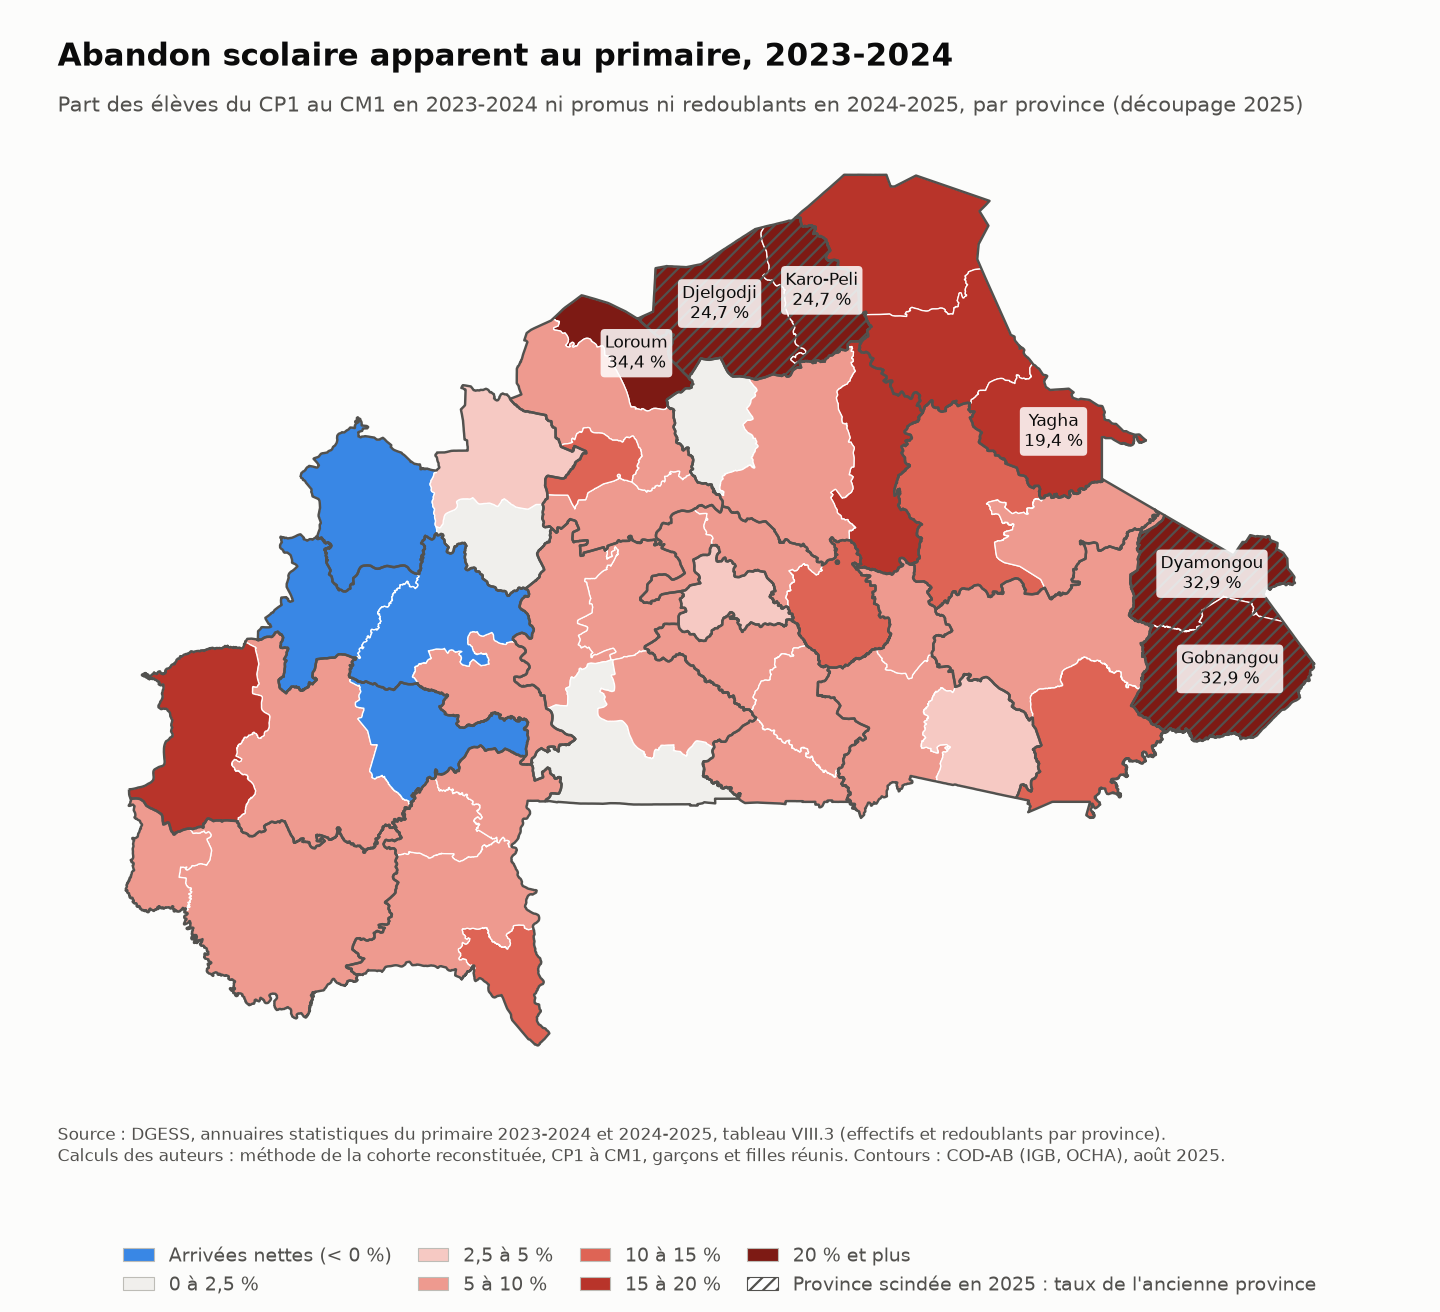
\includegraphics[width=\columnwidth]{fig_abandon_2023_2024.png}
\caption{Première carte issue de la base : abandon scolaire apparent au primaire en 2023-2024, par province (découpage 2025). Les deux provinces scindées reçoivent le taux de l'ancienne province. Source : DGESS, annuaires du primaire 2023-2024 et 2024-2025, tableau VIII.3 ; calculs des auteurs.}
\label{fig:abandon}
\end{figure}

%======================================================================
\section{Limites et anomalies signalées}
%======================================================================

Le nettoyage a révélé des anomalies dans les publications elles-mêmes. Elles sont consignées pour être transmises à leurs producteurs :
\begin{itemize}
\item dans l'annuaire du primaire 2024-2025, la répartition entre garçons et filles est impossible pour 31 provinces alors que le total est juste (par exemple 84\,353 filles pour 33\,313 garçons au CP1 du Kadiogo) ;
\item des étiquettes d'année absentes, erronées ou répétées dans l'historique des effectifs de plusieurs éditions, et un bloc imprimé deux fois (Mouhoun, édition 2024-2025) ;
\item des rapports ESU récents illisibles au niveau provincial et, depuis octobre 2023, l'absence de recensement des fermetures ;
\item un fichier de déplacés incomplet à la fin d'avril 2022 ;
\item dans le Data Pack, deux annuaires de l'éducation non formelle identiques sous deux noms (2019 et 2021, campagne 2020), et un troisième dont le nom (2020) ne correspond pas à la campagne (2019) ;
\item dans la base principale, des structures privées et communautaires du préscolaire apparemment interverties en 2019-2020 dans plusieurs régions, et des sauts brusques des effectifs et des structures du préscolaire en 2024-2025.
\end{itemize}

D'autres limites tiennent à la nature des données. Aucune donnée n'est disponible au niveau de l'école ou de l'élève. Les annuaires régionaux de l'INSD manquent pour le Centre-Est, le Centre-Nord et l'Est. Enfin, l'abandon calculé par différence d'effectifs mesure toutes les pertes nettes d'élèves d'une province : là où les écoles ferment ou rouvrent en masse, il cesse de mesurer le décrochage. Ces cas, repérés par une variation des effectifs supérieure à 30\,\% en un an, seront traités à part à l'étape de transformation.

%======================================================================
\section{Reproduction}
%======================================================================

La chaîne se relance depuis le dossier du projet, rangé dans le dossier des données des organisateurs, qui restent intactes. Elle demande Python 3.11 ou plus récent et les bibliothèques listées dans \texttt{requirements.txt} (pandas, geopandas, shapely, pyogrio, openpyxl, matplotlib). La commande \texttt{python -m sentinelle.collecte} produit les extractions et le dépôt 01 ; \texttt{python -m sentinelle.nettoyage} construit la base, rejoue les contrôles et produit le dépôt 02. Les notebooks \texttt{01\_collecte} et \texttt{02\_nettoyage} présentent les mêmes étapes avec leurs résultats. Les deux étapes s'exécutent en environ trois minutes.

\textbf{Usage d'outils d'intelligence artificielle.} Conformément au règlement~\cite{dcb_document}, un assistant de programmation a été utilisé pour écrire et relire le code de la chaîne de traitement. Les données traitées sont des statistiques publiques agrégées ; aucune donnée personnelle n'a été manipulée. Chaque résultat a été vérifié par les contrôles décrits ci-dessus et relu par l'équipe.

\bibliographystyle{named}
\bibliography{references}

\end{document}
